\chapter{Results}
\label{chapter3}

%<Results, evaluation (including user evaluation) {\em etc.} should be described in one or more chapters. See the `Results and Discussion' criterion in the mark scheme for the sorts of material that may be included here.>

\section{User Feedback} \label{section:user-feedback}

In order to evaluate the success of the solution produced, a method of collecting user feedback had to be developed. This was done by collecting a group of eligible testers who not only had relevant background to understand the material, but were also willing to devote time to the study and review the material. Then, a consistent and precise way of collecting the information had to be created so that a measurement of the success of the notebooks could be collected.

The information assessing the notebooks would be gathered through a series of questionnaires, one for each notebook, which were hosted on Google Forms. A link to the questionnaire can be found \href{https://docs.google.com/forms/d/175MU_wRfSiDJ0iOZruNCj8xvd4Ud7c0Js2M29bnK1PA/edit}{here}. In order to assess the success of the notebooks, the questions were tailored to points on the Learning Resource Requirements from Section \ref{section:learning-resource-requirements}. The survey consisted of a collection of questions aimed to assess how well these requirements were met and each question related to a specific requirement. Every question started with a description of the requirement in natural terms to give the tester appropriate background. Then they were asked to rate on a score of one to ten how well this objective was met. The final questionnaire can be seen in Appendix \ref{appendix:additional-pdfs} at the end of the report.

The only difference to the requirements laid out earlier is the inclusion of a question asking how interesting the content was. This was not included in the requirements since it is a fairly personal question. A user might find the content interesting because they find the subject itself interesting, regardless of the quality of writing. The opposite is also true. As such, this metric is not as important, although interesting to measure since there could still be some correlation between quality and interest. A more engaging and excitingly written resource would lead to the user finding the resource more interesting.

The scoring system is a simple one to ten score, the interpretations vary however. For most questions a higher score indicates a better result in terms of quality. This is not true for all questions, for instance ``How difficult was the content to understand?'' is question that ideally would be placed at a five or six.

\section{Notebook 1: Mathematical Review} \label{section:notebook-1}

We will now review the actual content produced. Each notebook starts with an introduction and a set of learning objectives that mirror those set out in the content plan. It is difficult here to give a complete description of each notebook, since it is a piece of written content and not code. The reader of this report is encouraged to view the notebooks themselves in the main repository.

\subsection{Section 1: Vector Spaces}

Notebook 1 Section 1 leads with vector spaces, a classic linear algebra topic. The definition of a field is introduced in order to further introduce the concept of a vector space. The reader is expected to recall the definition of a group and the axioms for a group are given in plain language, not given in mathematical notation. With these axioms and the additional axioms classifying a group as a vector space, the full definition is given. After this a few examples of vector spaces are given. In FEM, the only vector spaces we are concerned about are function spaces, but vector spaces are introduced more generally since the ideas of basis and linear independence are universal over all types of vector space. No check exercises were needed here.

\begin{figure}[h]
\centering
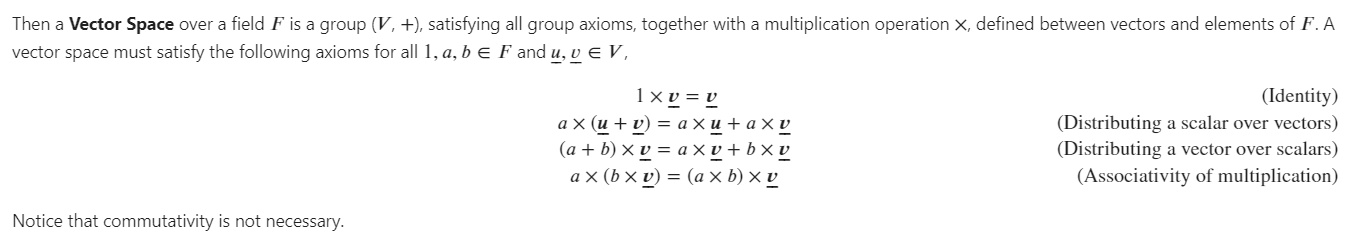
\includegraphics[width=\textwidth, frame]{./images/notebook1/1}
\end{figure}
Linear independence is the next subsection. The ideas of span, linear combinations and linear dependence are reviewed. A derivation is made that motivates the idea that a matrix whose columns consist of linearly independent vectors has a non-zero determinant. The check exercises consist of fairly simple questions testing the reader has understood linear independence. The first is to prove a set is linearly independent, which can be done by constructing the matrix and showing it has non-zero determinant. The other is to prove a set in linearly dependent. This is done by finding a linear combination of vectors that produce another vector in the set. This could be done by inspection or trial and error, but the example was written to be too difficult to be done this way, so instead the reader is encouraged to find the linear combination by Gaussian Elimination. 

The next subsection is about bases. The idea is introduced and then three examples are introduced. This is a fairly straightforward section. The check exercises here combine ideas from the previous sections, testing for analysis in Bloom's taxonomy. For instance, explaining why a set of vectors of size $n+1$ from a vector space of dimension $n$ cannot be linearly independent uses the idea of basis, dimension and linear independence.

\begin{figure}[h]
\centering
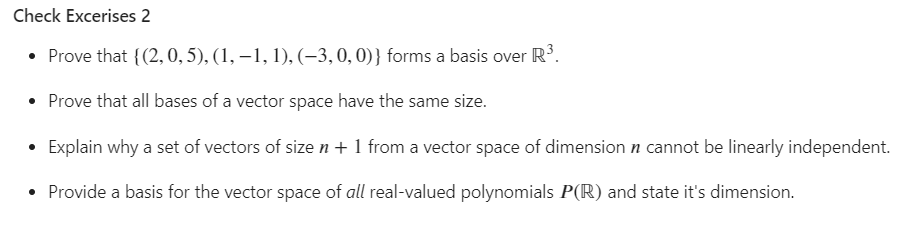
\includegraphics[width=0.7\textwidth, frame]{./images/notebook1/2}
\end{figure}

\subsection{Section 2: Vector Calculus}

This section aims to refresh students on vector calculus definitions, multiple integration and the divergence theorem. We start with a simple refresher on the idea of fields and mutlivariable functions, which leads directly into the idea of the partial derivative. The check exercises for this section ask the reader to state whether certain physical examples are vector or scalar fields. A second question tests the reader's differentiation skills by asking them to evaluate a partial derivative.

\begin{figure}[h]
\centering
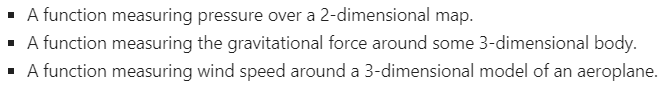
\includegraphics[width=0.7\textwidth, frame]{./images/notebook1/3}
\end{figure}

The next subsection refreshes the reader on a few common differential operators. Gradient is the most important one, but divergence is also very important and is used in most of our weak formulations
later on. A few paragraphs are devoted to explaining these and their interpretations in terms of fields. Curl and the Laplacian are also mentioned, since there are certain PDEs where these are useful. While explaining curl and its physical interpretation, a few diagrams are included. To finish the subsection, a question is asked about each of the differential operators introduced. The reader is asked to prove that gradient is a linear operator, to find the divergence of a field and ascertain whether it is incompressible, and to calculuate the curl of a field used in a previous exercise to verify it is irrotational.

The third subsection refers to multiple dimensional integration. It begins by discussing the idea of surface integrals over regions in the $xy$-plane. This is a precursor to the next point, which is on surface integrals over curved surfaces in three dimensional space. Volume integrals are mentioned, as a formula is presented that can be used to calculate a surface integral. This formula is not derived, but a derivation is not necessary at every stage since readers should still be familiar with these topics. Then an example of using this formula is run presented, where the function $f=1$ is integrated over the surface of a sphere, which derives the surface area of a sphere. To finish out the subsection, the idea of flux integrals are presented, although an example was not given since it won't be strictly necessary to compute them. The check exercises consist of several questions asking readers to calculate certain surface integrals. They are also given the cylindrical coordinate transformation and asked to use this to calculate the surface area of a cylinder, a classic example.

The final subsection discusses the Divergence Theorem and Green's Identities. These theorems are very useful for deriving variational forms for use with FEM, and are the whole reason so much attention was given to surface and flux integrals. The divergence theorem is presented without proof, while Green's first identity is derived from this. The final exercise asks the reader to derive Green's second identity, with the appropriate substitution they need to perform being given.

\section{Notebook 2: Introduction to the Finite Element Method}

\subsection{Section 3: Finite Element Method in 1D}

Notebook 2 is the first with new content. It opens with a section talking about the purpose of FEM and presents the example PDE that is solved throughout the notebook. Then, the first concept of a mesh is introduced, the simple one-dimensional case. The space of linear polynomials $P_1(I)$ is defined after this, along with its basis. This is the same course taken by Bengzon and Larson. Since the space of continuous piecewise linear polynomials is just a combination of linear polynomials, it makes sense to start at the most fundamental part, and build upwards. Then some visuals are presented illustrating the difference between continuous and discontinuous piecewise linear functions, which were created in Matplotlib. Finally, the space of piecewise continuous linear polynomials $V_h$ is presented, along with its basis of hat functions, which are key to understanding FEM. The exercises ask the reader to use knowledge from notebook 1 to prove the set of hat functions actually forms a basis on $V_h$. It then asks what its dimension would be on a mesh with $n+1$ nodes. 

\begin{figure}[h]
\centering
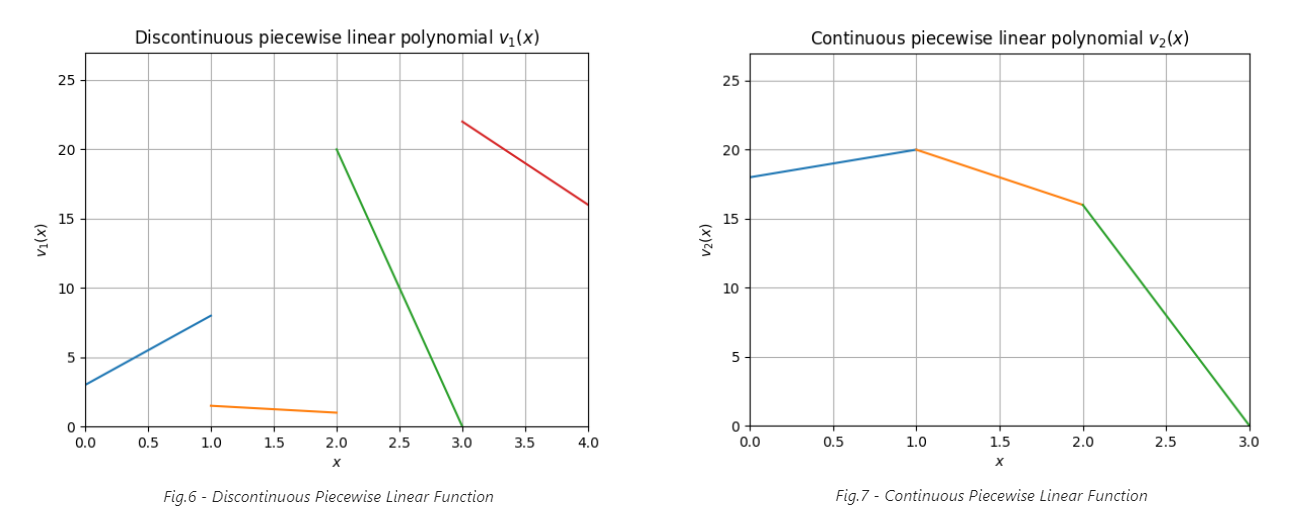
\includegraphics[width=0.7\textwidth, frame]{./images/notebook2/1}
\end{figure}

The next chapter is a bit more dense with information, it introduces the idea of the weak formulation and derives the formulation for the example equation presented in the introduction, the Poisson equation. A brief amount of time is spent explaining the classes of the function spaces involved. This is more to satisfy reader curiosity and provide a sense of completeness, but the actual functional analysis involved with defining these spaces properly is beyond the scope of this project. This allows us to produce our finite element approximated problem, similarly to Section \ref{subsection:how-fem-works}. The exercise here presents a simplified version of the one-dimensional heat equation called the steady state heat equation. The reader is asked to derive its variational form in the same way as the example.

The next subsection is short, it moves from the variational form to a system of linear equations through some derivations. The derivation is the same as the one used in Bengzon-Larson, with some extra lines added for additional clarity. The exercise asks the reader to derive the system of linear equations for the steady state heat equation.

\begin{figure}[h]
\centering
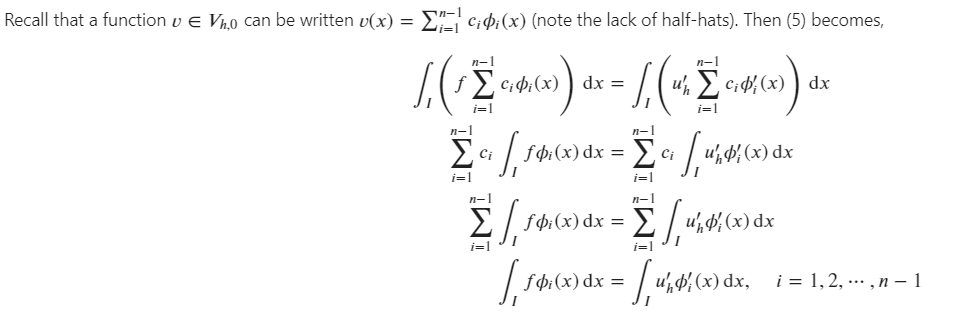
\includegraphics[width=0.7\textwidth, frame]{./images/notebook2/2}
\end{figure}

Finally, the section ends with a complete example, solving a very simple one dimensional differential equation. This example can be solved analytically by simply integrating twice and fixing boundary conditions. The reason for such simplicity is to provide a way of comparing the accuracy and showing that the method does, in fact, work. A mesh of three cells is used to calculate the finite element approximation by hand. This is then plotted against the analytical solution using Matplotlib. Then some additional points are mentioned about the convergence of FEM, types of quadrature, linear equation solvers and higher dimensional piecewise continuous function spaces.

\begin{figure}[h]
\centering
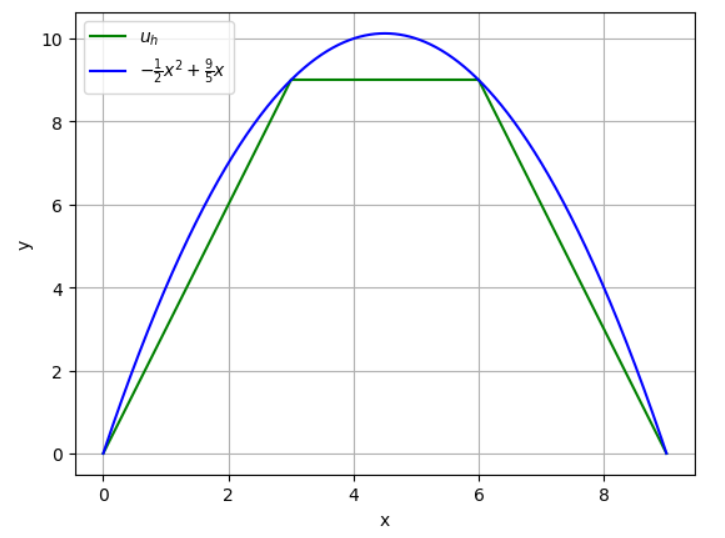
\includegraphics[width=0.5\textwidth, frame]{./images/notebook2/3}
\end{figure}

\subsection{Section 4: Finite Element Method in 2D}

The subsections here mostly parallel Section 3. We start with an introduction to piecewise polynomial functions of two variables although we skip the more intricate definitions in favour of a blunt approach, since the method of understanding the two are very similar. The real idea of a mesh is introduced and some FEniCSx code is presented that generates a mesh over a circle and visualises it with Pyvista.

After this, the variational form is defined for the two dimensional Poisson equation, here using Green's first identity derived in the previous notebook. Then, as before, the linear system is constructed. The final subsection of the 2D portion discusses boundary conditions and modelling. The concepts of Dirichlet, Neumann, and Robin boundary conditions are introduced and explained. The strengths and weaknesses of FEM are presented as well as the final steps for performing it.

\begin{figure}[h]
\centering
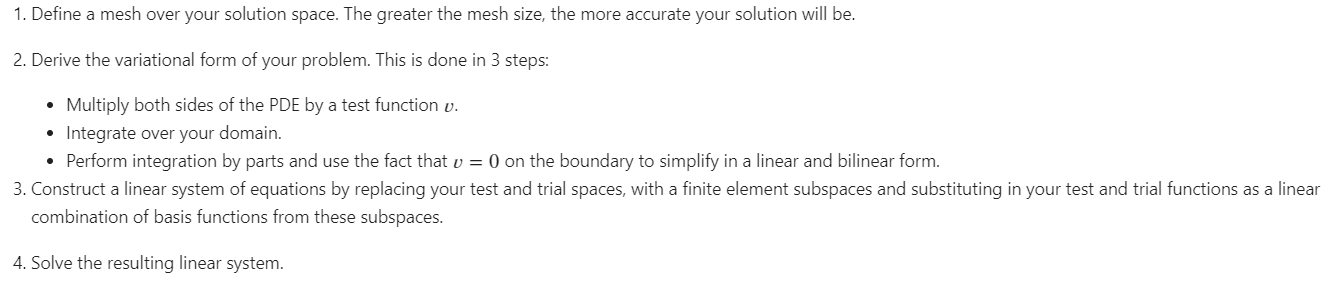
\includegraphics[width=0.9\textwidth, frame]{./images/notebook2/5}
\end{figure}

\subsection{Section 5: Time Dependent Problems}

This short section aims to introduce the idea of time dependent problems in theory, for practical implementation later. The example presented is the 2D heat equation with Dirichlet boundary conditions.

\begin{align*}
\frac{\partial u}{\partial t} &= \nabla^2u + f \quad& x\in\Omega, \, t\in [0,T] \\
u &= u_D \quad& x \in \delta\Omega, \, t\in [0,T] \\
u &= u_0 \quad& t=0
\end{align*}

The method presented is called the backwards Euler method, where time is discretised and a difference quotient is used to approximate the derivative.

\begin{figure}[H]
\centering
\begin{tabular}{cc}
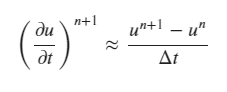
\includegraphics[width=0.2\textwidth, frame]{./images/notebook2/6} &   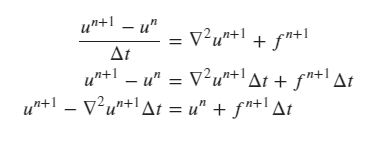
\includegraphics[width=0.4\textwidth, frame]{./images/notebook2/7} 
\end{tabular}
\end{figure}

The variational form is not derived, but the finite difference approximation is. Then finally, the processes of interpolation and $L^2$ projection are discussed. This is necessary because when solving a system with an initial condition using Euler's method and FEM, the initial condition has to be from the same space as the solution and so must be approximated in that space. This is done via these techniques. The final exercise asks the reader to complete the derivation of the variational form of the two-dimensional heat equation. A challenge that brings together all the work done so far, but definitely within the realm of understanding.

\section{Notebook 3: Implementing FEM in Python with FEniCSx}

\subsection{Section 6: Introduction to FEniCSx}

The final notebook intends to show readers how to implement some simple equations in the previously finite element computing platform FEniCSx. It begins with an introduction to FEniCSx and each of its main constituent libraries as in Section \ref{subsection:overview-of-tools}. The section will be devoted to solving the following instance of the Poisson equation.

\begin{align}
-\nabla^2 u(x,y) &= f = 5y^{-\frac32} - 1 \quad &\text{in } \Omega \\
 u(x,y) &= u_D = 20y^\frac12 + \frac12 x^2 + 2x \quad &\text{on } \delta\Omega, \\
 \text{where } \delta\Omega &= [0,1] \times [0,1]
\end{align}

This BVP was created using the method of manufactured solutions, a method that guarantees an analytical solution will exist. The solution was designed so that the boundary condition is the solution. As before, this is so we can compare our approximated solution to the one produced. The majority of the code is adapted from Dokken's tutorial but has been changed to fit the example presented. A further degree of complexity has been added to the problem from Dokken's example by the inclusion of fractional powers.

First, the boundary is defined as the unit square in Gmsh. Code performing this is shown, along with a block creating a visualisation in Pyvista. Next, all the problem parameters are defined, including the function spaces, boundary conditions, test and trial functions, linear and bilinear terms in UFL and the PETSc linear problem solver. Intuitive explanations are given every step of the way. A few paragraphs are also given to the numerical methods happening behind the scenes, with attention being given to LU Factorisation. With the problem wholly defined, it is then easy to solve using PETSc.

With the equation solved, the next thing to teach was how to visualise the solution obtained. This was done over a few methods. Firstly, Pyvista was used. The approach was the exact same as visualising the mesh earlier, the difference being that the nodes are coloured based on the values of the degrees of freedom of the approximated solution. This plotter can then be extended to three dimensional space with the \texttt{warp\_by\_scalar()} method.

\begin{figure}[H]
\centering
\begin{tabular}{cc}
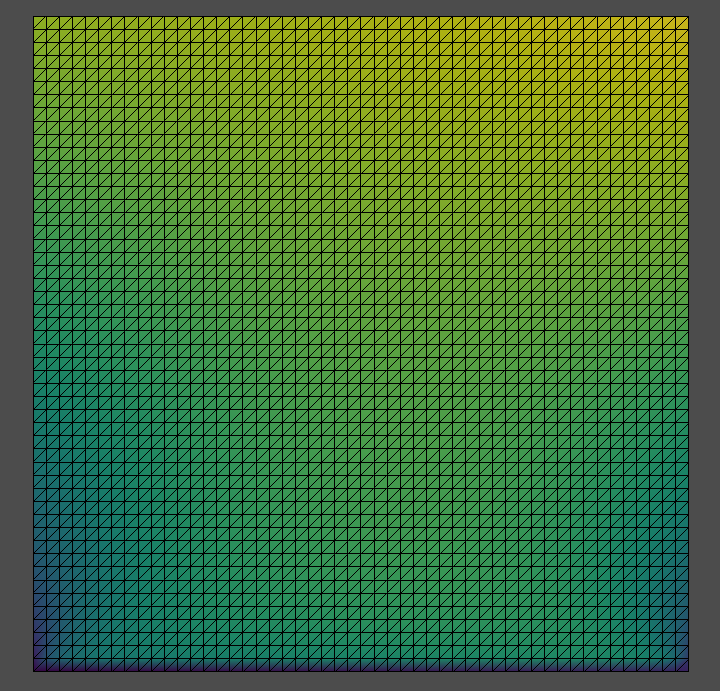
\includegraphics[width=0.3\textwidth, frame]{./images/notebook3/1} &   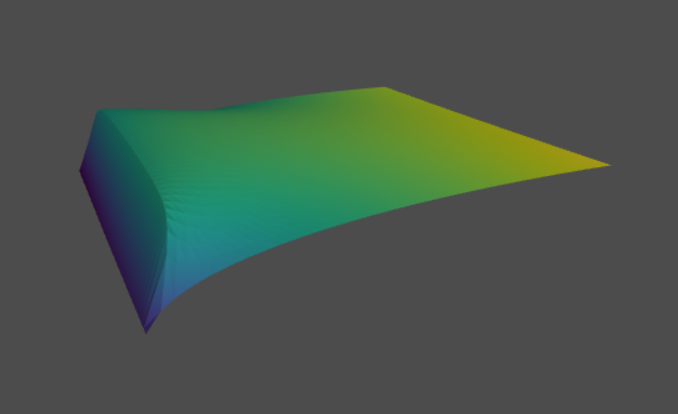
\includegraphics[width=0.4\textwidth, frame]{./images/notebook3/2} 
\end{tabular}
\end{figure}

The other method of visualisation presented was by plotting the value of the function along a straight line through the domain, a so called "slice" of the function. This method is covered by Dokken in his elastic deformation chapter, but is used here in a different context with much more explanation. The process can be broken down into three steps: 1. Define all the points on the line $x=0.5$ (the middle of the domain). 2. Evaluate the approximate solution at these points. 3. Plot these values against the points on the line.

Numpy's array manipulation techniques are first used to define the points on the line. DOLFINx's way of evaluating the function over a set of point efficiently involves the use of Axis Aligned Bounding Boxes. A detailed description of the algorithms and data structures involved is given, with this Azure From The Trenches post \cite{aabb-tree} being the main source. 

\begin{figure}[h]
\centering
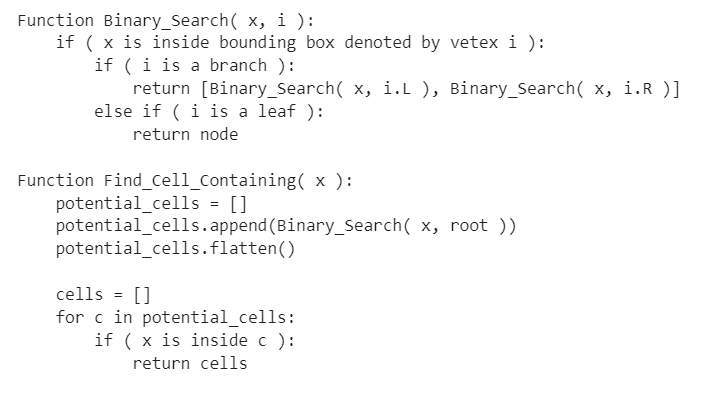
\includegraphics[width=0.6\textwidth, frame]{./images/notebook3/3}
\end{figure}

Then, with $u_h$ evaluated over the points, the curve is plotted in Matplotlib. This process was repeated multiple times with varying mesh sizes to demonstrate the convergence to a final solution. This was then compared to the analytical solution to show readers that the solution is correct. Finally, the complete set of steps for solving a BVP in FEniCSX is summarised and an exercise is presented asking readers to solve an instance Poisson equation in FEniCSX.

\subsection{Section 7: A Time Dependent Example}

The final section of the final notebook is devoted to solving a time dependent problem in FEniCSx. This chapter aims to illustrate the power and versatility of FEniCSx. The first subsection introduces the problem to be solved, the wave equation. This is based on Dokken's tutorial on the heat equation, but has been adapted for a different example. The main difference between the heat equation and the wave equation is that the heat equation contains a first order derivative with respect to time, while the wave equation contains a second order derivative. This means in approximating with a difference quotient, a second order one must be used, which changes the structure of the problem. The first subsection introduces the instance to be solved, and derives the linear and bilinear terms from this.

\begin{figure}[h]
\centering
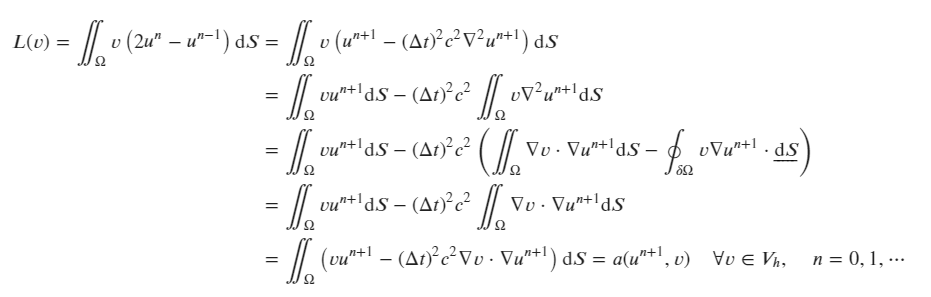
\includegraphics[width=0.8\textwidth, frame]{./images/notebook3/6}
\end{figure}

The final subsection contains the implementation. The problem is defined in FEniCSx, along with all parameters such as time-step size, mesh size and some constants in the equation. Everything is mostly the same as the previous section until we reach the point of solving. Instead of constructing a linear problem like before, a linear problem needs to be created at every time step. If one were to create such a large number of new PETSc linear problems, the performance impact would be quite considerable. Instead a more clever approach is used by noticing that the mass matrix stays constant throughout all the linear problems. FEniCSx has functionality built in to allow the mass matrix and load vector to be built separately, so only the load vector is built at each time step.

The implementation of this is shown, and to visualise this time dependent solution, every frame is rendered into a \texttt{.gif} file. The result is an animation, of which one frame can be seen below.

\begin{figure}[h]
\centering
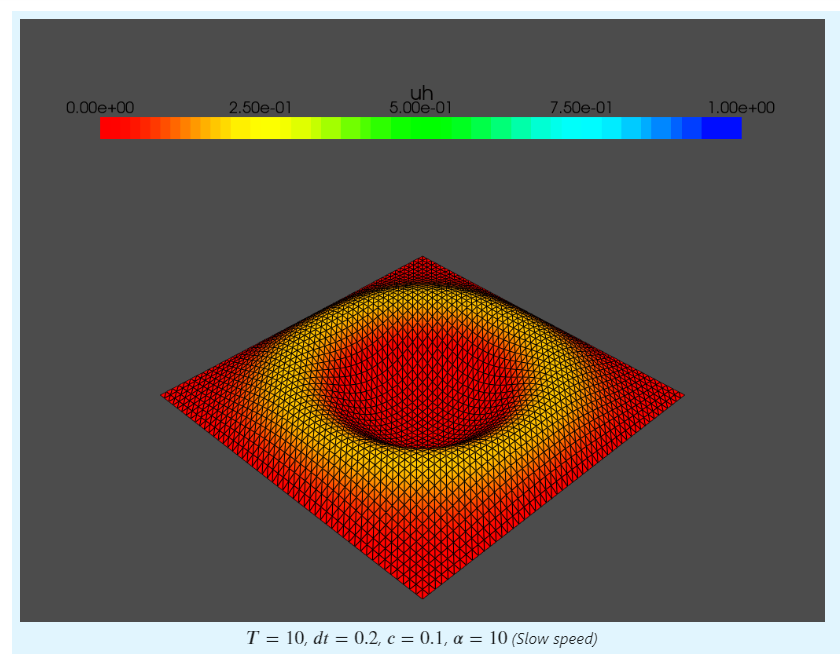
\includegraphics[width=0.4\textwidth, frame]{./images/notebook3/7}
\end{figure}

Four example animations are presented with different parameters, but the reader is encouraged to experiment to see what other kinds of interesting instances they can produce. The final exercise asks the user to create a finite element approximation to an instance of the heat equation of their choosing. A fitting end since if they can complete this exercise, they will have successfully create their own finite element approximation from start to finish!